\documentclass[11pt]{article}
\usepackage[T1]{fontenc}
\usepackage{lmodern,amsmath,amssymb,amsthm}
\usepackage[margin=1.04in]{geometry}
\usepackage{tikz}
\usepackage[hidelinks]{hyperref}
\newtheorem{theorem}{Theorem}
\newtheorem{lemma}[theorem]{Lemma}
\newcommand{\area}[1]{\lvert #1\rvert}
\newcommand{\tri}[3]{\triangle #1#2#3}
\title{The sharp area ratio for a largest inscribed triangle with a side on the boundary}
\author{}
\date{}
\begin{document}
\maketitle
\vspace{-2.5em}
\begin{abstract}
Let $T$ be a largest-area triangle in a planar convex body $K$.
If a whole side of $T$ lies on the boundary of $K$, the largest possible
value of $\area K/\area T$ is $\pi-4\arctan t-t^2=2.3075689464\ldots$,
where $(1+t)^4=2(1+t^2)$ and $0<t<1/4$.
This answers Problem 3.4 of Erd\H{o}s, Purdy and Straus (1982).
We construct an attaining body with elliptic arcs. The proof pairs
horizontal sections by an involution. The same involution certifies the
upper bound for every body, including bodies with no symmetry.
\end{abstract}

\section{The problem}

Write $M(K)$ for the largest area of a triangle contained in a compact
convex set $K\subset\mathbb R^2$ with interior. Such a triangle exists
by compactness. Without a restriction on its edges, the sharp bound is
$\area K/M(K)\le4\pi/(3\sqrt3)$, with equality for ellipses
\cite[Theorem 1.2]{EPS}. Problem 3.4 of Erd\H{o}s, Purdy and Straus
asks for the sharp bound when a largest triangle has a side on
$\partial K$ \cite[p.~52]{EPS}.

\begin{theorem}\label{main}
Let $t$ be the unique root of $(1+t)^4=2(1+t^2)$ in $(0,1/4)$.
If there is a largest triangle in $K$ with a side contained in
$\partial K$, then
\[
 \frac{\area K}{M(K)}\le \pi-4\arctan t-t^2.
\]
Some convex body attains this bound and has a largest triangle with
exactly one side contained in its boundary.
\end{theorem}

The sharp constant for pentagons is $\sqrt5$. Fleischer, Mehlhorn, Rote,
Welzl and Yap exhibited a hexagon of ratio $9/4$ whose largest triangle
has a boundary side \cite[Appendix, Lemma A.4]{FMRWY}. Thus the
pentagon bound was already known to fail for general bodies. The issue
in Problem~3.4 is to determine the sharp value. Section~\ref{history}
describes the relation with the finite-polygon and line-transversal results.

\section{A necessary inequality for widths}\label{necessary}

Choose a largest triangle $ABC$ with $AB\subset\partial K$. Apply an
invertible affine map that sends $A,B,C$ to $(-1/2,0),(1/2,0),(0,1)$.
All areas change by the same factor, so $M(K)=1/2$ in these coordinates.
A support line at the midpoint of $AB$ contains $A,B$, since the
midpoint attains the maximum of a supporting linear functional. Thus
$K$ lies in $y\ge0$. A point above $y=1$ gives a larger triangle on
base $AB$. A point on $y=0$ outside $AB$ gives a larger triangle on
that line with vertex $C$. It follows that the heights are $[0,1]$ and
the full base section is $AB$.

Write $[l(y),r(y)]$ for the interval of horizontal coordinates of the
section at height $y$, and put $f(y)=r(y)-l(y)$. These endpoints
exist and the intervals are nonempty because $K$ is compact and contains
the normalized triangle. Convexity makes $l$ convex and $r$ concave on
the open height interval. In particular the bounded section widths are
measurable, and $\area K=\int_0^1 f(y)\,dy$.

\begin{lemma}\label{widthbound}
Whenever $0\le y\le z\le1$,
\begin{equation}\label{constraint}
 z-y+zf(y)+yf(z)\le2 .
\end{equation}
In particular $f(y)\le1+y$.
\end{lemma}
\begin{proof}
For points $(b,0),(u,y),(v,z)$ the oriented double area is
$zu-yv-(z-y)b$. Choose $(b,u,v)=(-1/2,r(y),l(z))$ and
$(1/2,l(y),r(z))$ in turn. Their double areas belong to $[-1,1]$.
Their difference is the left side of \eqref{constraint}.
Set $z=1$ and use $f(1)\ge0$ for the last assertion.
\end{proof}

\section{The extremizing body}\label{attainment}

Expanding the parameter equation gives
$t^4+4t^3+4t^2+4t-1=0$. This polynomial is strictly increasing on
$[0,\infty)$ and has opposite signs at $0$ and $1/4$. Define
\[
 R=1+t^2,\qquad m=\frac{(1+t)^2}{2}=\sqrt{R/2},\qquad
 s(y)=\sqrt{R-y^2}\quad(t\le y\le1).
\]
Then $t<m<1$. The map $s$ decreases from $1$ to $t$,
$s(s(y))=y$, and $s(m)=m$. Put
\begin{equation}\label{candidate}
 w(y)=
 \begin{cases}
  1+y,&0\le y\le t,\\[2pt]
  2s(y)/R-\lvert 1-y/m\rvert,&t\le y\le1,
 \end{cases}
 \qquad K_* = \{(u,y):0\le y\le1,\ |u|\le w(y)/2\}.
\end{equation}
At $t$ the second expression equals $1+t$. Its right derivative is
$-2t/R+1/m=1$, since $R=2m^2$ and $2m-2t=R$.
At $1$ the second expression is zero by the same identities.
The function $s$ has second derivative $-R/(R-y^2)^{3/2}$, and
$-|1-y/m|$ is concave. The two pieces of $w$ meet with the same
slope at $t$, so $w$ is continuous and concave on $[0,1]$.
Its endpoint chord and its first linear piece therefore give
\begin{equation}\label{sandwich}
 1-y\le w(y)\le1+y \qquad (0\le y\le1).
\end{equation}
The region $K_*$ is compact, convex, and has interior. Its left and
right boundaries consist of line segments and affine images of circular
arcs, since $s(y)^2+y^2=R$ and the absolute value is piecewise linear.

\begin{lemma}\label{admissible}
The normalized triangle with base $AB$ and apex $C$ is a largest triangle
of $K_*$. Its base is its only side contained in $\partial K_*$.
\end{lemma}
\begin{proof}
For three points at heights $x\le y\le z$, the coefficients of their
horizontal coordinates in the oriented double area have absolute values
$z-y$, $z-x$ and $y-x$. Since the sections are centered intervals,
the largest absolute double area at these heights is
\[
 \tfrac12\big((z-y)w(x)+(z-x)w(y)+(y-x)w(z)\big).
\]
The difference of the expression in parentheses and its value at $x=0$ is
$(z-y)(w(x)-1)-x(w(y)+w(z))$. This is at most zero:
\eqref{sandwich} gives $w(x)-1\le x$ and
$w(y)+w(z)\ge1-y\ge z-y$. It suffices to verify
\eqref{constraint} for $w$ at every pair $y\le z$.

If $t\le y\le z$, Cauchy--Schwarz applied to
$(z,s(z))$ and $(s(y),y)$ gives $zs(y)+ys(z)\le R$. Also
\[
 z\lvert1-y/m\rvert+y\lvert1-z/m\rvert
 \ \ge\ \lvert z(1-y/m)-y(1-z/m)\rvert=z-y.
\]
Substitution in \eqref{candidate} proves \eqref{constraint}.
For $y\le m$ and $z=s(y)$, both inequalities are equalities:
the two vectors coincide, and $y\le m\le z$.
If $y<t\le z$, the left side of \eqref{constraint} is
$2z+y(z-1+w(z))$. Its coefficient of $y$ is nonnegative by
\eqref{sandwich}, so its value at $y=t$ is an upper bound.
If $z<t$, the expression is $2z(1+y)\le2t(1+t)<2$.
These cases bound every triangle by $1/2$, the area of $ABC$.
At height $t$, its other sides have horizontal coordinates
$\pm(1-t)/2$. Both points are interior to $K_*$ because
$w(t)=1+t$ and the profile is continuous. The base is on the
support line $y=0$.
\end{proof}

\begin{figure}[ht]
\centering
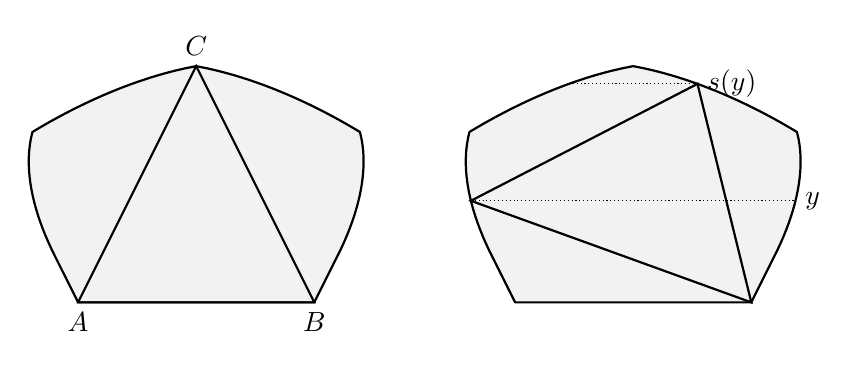
\begin{tikzpicture}[x=3.0cm,y=3.0cm,thick,
  declare function={
    tp=0.201045931; rp=1+tp^2; mp=(1+tp)^2/2;
    halfwidth(\y)=(2*sqrt(rp-\y^2)/rp-abs(1-\y/mp))/2;
  }]
  \foreach \offset in {0,1.85} {
    \begin{scope}[shift={(\offset,0)}]
      \path[draw,fill=black!5,line join=round]
        (-.5,0)--(.5,0)--({(1+tp)/2},{tp})
        -- plot[variable=\y,domain=tp:mp,samples=20] ({halfwidth(\y)},\y)
        -- plot[variable=\y,domain=mp:1,samples=30] ({halfwidth(\y)},\y)
        -- plot[variable=\y,domain=1:mp,samples=30] ({-halfwidth(\y)},\y)
        -- plot[variable=\y,domain=mp:tp,samples=20] ({-halfwidth(\y)},\y)
        --cycle;
    \end{scope}}
  \draw (-.5,0) node[below] {$A$} -- (.5,0) node[below] {$B$}
    -- (0,1) node[above] {$C$} --cycle;
  \begin{scope}[shift={(1.85,0)}]
    \def\lowerheight{0.43}
    \pgfmathsetmacro{\upperheight}{sqrt(rp-\lowerheight^2)}
    \draw[densely dotted,thin] ({-halfwidth(\lowerheight)},\lowerheight)
      --({halfwidth(\lowerheight)},\lowerheight) node[right] {$y$};
    \draw[densely dotted,thin] ({-halfwidth(\upperheight)},\upperheight)
      --({halfwidth(\upperheight)},\upperheight) node[right] {$s(y)$};
    \draw (.5,0)--({-halfwidth(\lowerheight)},\lowerheight)
      --({halfwidth(\upperheight)},\upperheight)--cycle;
  \end{scope}
\end{tikzpicture}
\caption{Two triangles of maximum area in the same extremizing body.
The left triangle has a boundary side. The right triangle realizes equality
in \eqref{constraint} at two paired heights.}
\label{fig:paired}
\end{figure}

\section{An upper bound with equality}\label{optimality}

Let $K$ be any normalized admissible body, with section width $f$.
Set $D=f-w$. By Lemma~\ref{widthbound}, $D\le0$ on $[0,t]$.
For each $y\in[t,1]$, apply \eqref{constraint} to the heights $y,s(y)$
in increasing order. Lemma~\ref{admissible} gives equality for $w$
at this pair, also when $s(y)\le y$ by the involution. The difference is
\[
 s(y)D(y)+yD(s(y))\le0 .
\]
Since $s(y)\ge t>0$ and $s'(y)=-y/s(y)$, the substitution $z=s(y)$
gives
\[
 \int_t^1 D(y)\,dy
 \le -\int_t^1 \frac{y}{s(y)}D(s(y))\,dy
 = -\int_t^1 D(z)\,dz .
\]
Thus $\area K\le\int_0^1w=\area{K_*}$. The proof uses only the widths
of the sections of $K$ and places no condition on their centers.

For the value of the integral, a primitive of $2s(y)/R$ is
$\arcsin(y/\sqrt R)+ys(y)/R$. The algebraic term has the same value
at $t$ and $1$. The two angles there are $\arctan t$ and
$\pi/2-\arctan t$. The other term integrates to
\[
 \int_t^1 |1-y/m|\,dy
 =\frac{(m-t)^2+(1-m)^2}{2m}
 = 2m-1-t,
\]
using $1+t^2=2m^2$. Adding $\int_0^t(1+y)\,dy=t+t^2/2$
and substituting $2m=(1+t)^2$ yields
\[
 2\int_0^1w(y)\,dy=\pi-4\arctan t-t^2.
\]
This proves Theorem~\ref{main}. For comparison with $9/4$ without relying
on numerical rounding, the parameter polynomial is positive at $21/100$.
Thus $t<21/100$, and $\arctan t<t$ and $\pi>3.14$ imply
$\pi-4\arctan t-t^2>2.2559>9/4$.

\section{Pentagons, hexagons, and line transversals}\label{history}

Straus asserted $\area K/M(K)\le\sqrt5$ under the boundary-side
hypothesis \cite[Lemma 2, p.~309]{Straus}. The value is correct for
pentagons. We give the details of the finite-polygon comparison because
it identifies the valid application of this assertion in later work.

For a polygon, some largest triangle has all its vertices among the
vertices of the polygon: its oriented area is affine in each vertex.
In the extremal-pentagon argument of Fleischer et al.\ \cite[Lemmas
A.1--A.4 and the proof of Theorem A.6]{FMRWY}, one may choose a
largest-ratio instance among polygons with at most five vertices in
which every vertex belongs to at least two largest vertex triangles.
Indeed a vertex in only one such triangle can be displaced along a line
preserving its area, in a direction that does not decrease the
polygon's area, until another triangle ties or a vertex disappears.
A vertex in no such triangle can increase the area. Compactness after
affine normalization, followed by minimizing the number of vertices
and maximizing the number of tied triangles, gives the assertion.
A largest triangle through three consecutive vertices bounds the
ratio by two, by the two supporting strips along its incident sides
\cite[Lemma A.2]{FMRWY}. A triangle or quadrilateral also has ratio
at most two (split the latter along a diagonal).

It remains to consider a pentagon with at least four tied largest
triangles, each using two of its five diagonals. Two triangles
therefore share a diagonal. If their third vertices lie on opposite
sides, the two triangles force a parallelogram of ratio two
\cite[Lemma A.3]{FMRWY}. In the remaining case label the consecutive
vertices $A,B,C,D,E$ so that $ABD$ and $ACD$ are largest. After an
affine change of coordinates put
$A=(0,0),B=(0,1),C=(\delta,1),D=(1,0),E=(u,-v)$.
Here $0<\delta\le1$, since $ABC$ has double area $\delta$.
The triangles $BDE$, $ACE$ and $BCE$ give, respectively,
\[
  v\le u,\qquad u+\delta v\le1,\qquad \delta(1+v)\le1 .
\]
Consequently $v\le\min\{1/(1+\delta),1/\delta-1\}$. The pentagon
has ratio $1+\delta+v$. Put $g=(\sqrt5-1)/2$. For $\delta\le g$
the bound $1+\delta+1/(1+\delta)$ increases to $\sqrt5$.
For $g\le\delta\le1$ the bound $\delta+1/\delta$ decreases from
$\sqrt5$. A regular pentagon gives equality, as one sees by taking a
triangle cut out by two diagonals and one side. The equality case
up to affine maps is also recorded after Lemma A.4 in \cite{FMRWY}.

Fleischer et al.\ give a six-vertex example of ratio $9/4$
\cite[Lemma A.4, Case 2 and Fig.~13]{FMRWY}. In their coordinates
at $\delta=2/3$, scaled by six, the vertices in boundary order are
\[
 (0,0),\ (0,6),\ (4,6),\ (6,0),\ (4,-3),\ (3,-3).
\]
The shoelace sum has absolute value $81$. Label the vertices from $A$
to $F$. For vertex triples in lexicographic order, the largest absolute
determinants with first vertex $A,B,C,D$ are $36,36,24,3$,
respectively. Triangle $ABD$ attains $36$ and shares precisely $AB$
with the boundary. Its ratio $81/36=9/4$ is greater than $\sqrt5$.
Their Theorem A.6 proves that $9/4$ is the maximum over all convex
polygons with at most six vertices, even without imposing a boundary
side. Their example thus already refutes the unrestricted form of
Straus's lemma.

Jer\'onimo-Castro and Rold\'an-Pensado repeated that form as Lemma~S
\cite[p.~337]{JCRP}. In Claim~1 of their proof of Theorem~3,
$A,B,C,D,E$ are the vertices of a convex pentagon and $ABD$ is a
largest triangle. They use only
\[
 \area{DBC}+\area{DAE}+\area{ABD}\le\sqrt5\,\area{ABD}.
\]
The left side is the area of that pentagon. Its proved bound above
supplies precisely this inequality. Their conclusion
$\lambda(K,4)\le(1+\sqrt5)/2$ therefore holds with the restricted
lemma. Here $\lambda(K,4)$ is the dilation factor for a common line
transversal to a finite family of translates of $K$ when every four
members have one.

\paragraph{Proof verification and acknowledgments.}
OpenAI Codex developed the mathematical proof and its Lean
formalization. The formal theorem constructs an attaining body, bounds
all other admissible bodies, and checks the integral. Its source and
reproduction instructions are available in the public research
repository \cite{Lean}. Edgardo Rold\'an-Pensado reviewed the argument,
believes the sharp bound is correct, and confirmed that the pentagon
bound suffices for Theorem~3 despite the general error in Lemma~S.

\begin{thebibliography}{9}
\bibitem{EPS}
P.~Erd\H{o}s, G.~Purdy and E.~G.~Straus.
On a problem in combinatorial geometry.
\emph{Discrete Mathematics} \textbf{40} (1982), 45--52.
\href{https://users.renyi.hu/~p_erdos/1982-09.pdf}{Author archive}.
\bibitem{FMRWY}
R.~Fleischer, K.~Mehlhorn, G.~Rote, E.~Welzl and C.~Yap.
Simultaneous inner and outer approximation of shapes.
\emph{Algorithmica} \textbf{8} (1992), 365--389.
\href{https://doi.org/10.1007/BF01758852}{doi:10.1007/BF01758852}.
\bibitem{JCRP}
J.~Jer\'onimo-Castro and E.~Rold\'an-Pensado.
Line transversals to translates of a convex body.
\emph{Discrete \& Computational Geometry} \textbf{45} (2011), 329--339.
\href{https://doi.org/10.1007/s00454-010-9293-9}{doi:10.1007/s00454-010-9293-9}.
\bibitem{Straus}
E.~G.~Straus. Some extremal problems in combinatorial geometry.
In \emph{Combinatorial Mathematics}, Lecture Notes in Mathematics
\textbf{686}, Springer (1978), 308--312.
\href{https://doi.org/10.1007/BFb0062546}{doi:10.1007/BFb0062546}.
\bibitem{Lean}
\emph{Erd\H{o}s--Purdy--Straus, Problem 3.4}. Lean 4 formalization,
PR~81, November 2026.
\href{https://github.com/aliromman/math/pull/81}{Repository and verification}.
\end{thebibliography}
\end{document}
